\section{Aufbau}
\label{sec:Aufbau}

\begin{figure}
	\centering
	\caption{Die Plandarstellung einer realen Photodiode.}
	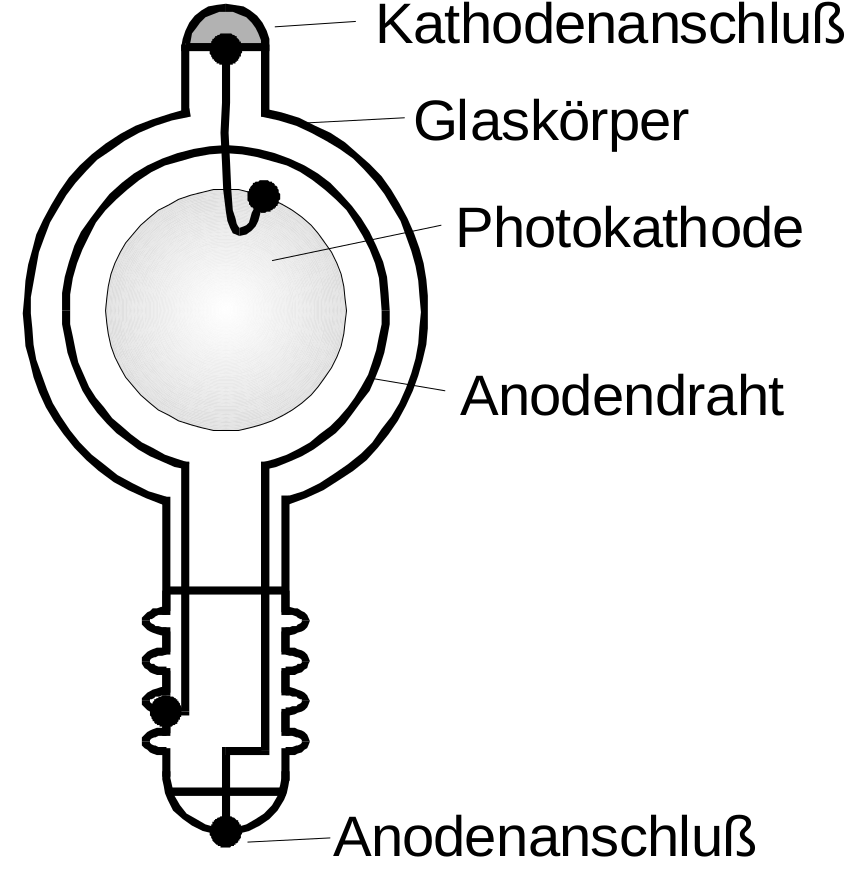
\includegraphics[width=\linewidth-280pt,height=\textheight-280pt,keepaspectratio]{content/Bilder/Photodiodereal.png}
	\label{fig:photodiodereal}
\end{figure}
\begin{figure}
	\centering
	\caption{Der optische Teil des Versuchsaufbaus.}
	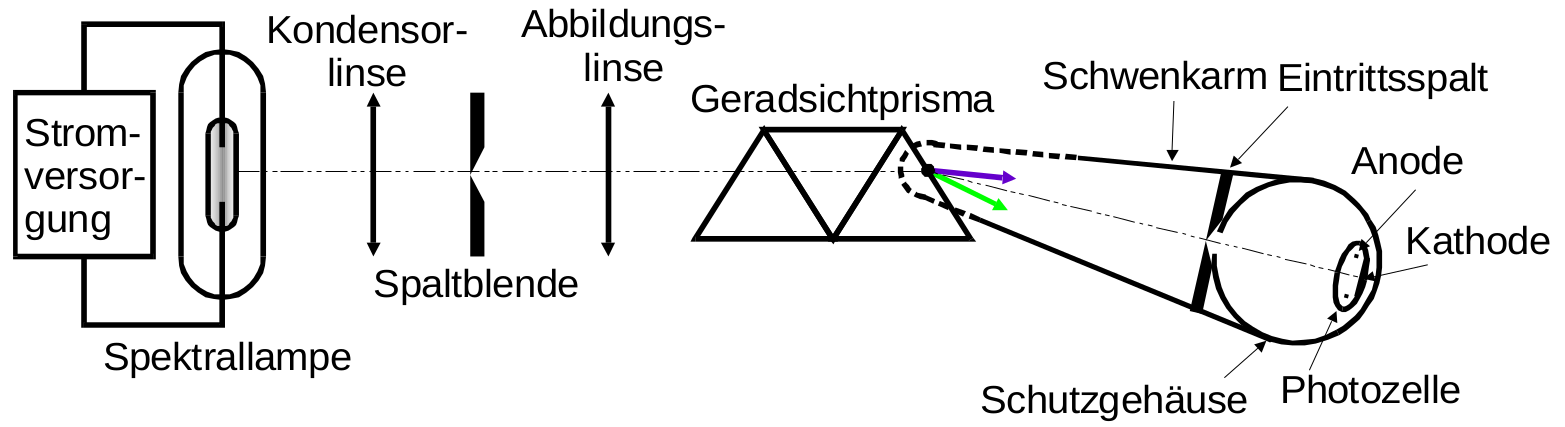
\includegraphics[width=\linewidth-70pt,height=\textheight-70pt,keepaspectratio]{content/Bilder/Optikteil.png}
	\label{fig:optikteil}
\end{figure}
\begin{figure}
	\centering
	\caption{Die Schaltung des elektrischen Teiles des Versuchaufbaus.}
	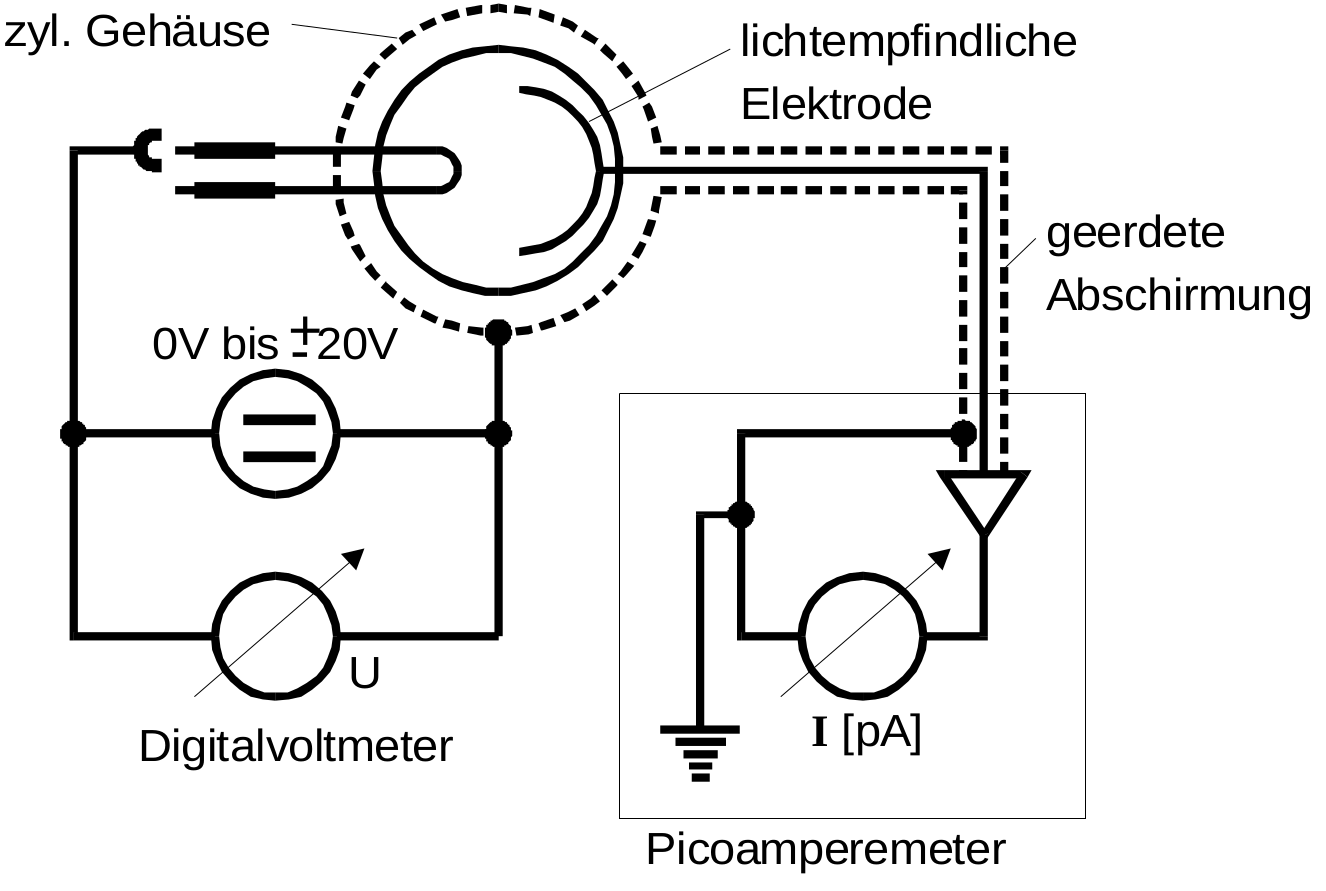
\includegraphics[width=\linewidth-150pt,height=\textheight-150pt,keepaspectratio]{content/Bilder/Elektrikteil.png}
	\label{fig:elektrikteil}
\end{figure}





Der Messaufbau besteht aus zwei Teilen. Zum einen wird ein optischer Aufbau verwendet \ref{fig:optikteil} ,
in welchem das Licht der Quecksilber Lampe in seine monochromatischen Spektrallinien
aufgespalten wird. Zum anderen wird eine Schaltung mit einer Photodiode verwendet \ref{fig:elektrikteil} um die auftretenden
Effekte in Form einer Stromstärkenänderung sichtbar zu machen. Der optische Aufbau
besteht zunächst aus der Lampe, deren Licht mit einer Kondensorlinse gebündelt wird.
 Mithilfe eines Einzelspaltes wird der Lichtstrahl in seine Spektrallinien zerlegt.
 Diese werden anschließend mit einer Abbildungslinse auf den Eintrittsspalt der
 Photokathode geworfen. Zuletzt wird eine Geradsichtprisma verwendet um die
 einzelnen Linien räumlich zu trennen. Die Photodiode besteht aus der bestrahlten
 Photokathode und einer ringförmigen Photoanode, welche um die Kathode gelegt ist \ref{fig:photodiodereal}
 Zwischen beiden liegt eine variierbare Beschleunigungsspannung an. Die vorherrschende
 Stromstärke wird mit einem geerdeten Pikoamperemeter gemessen.
